\documentclass[12pt,a4paper]{article}
\usepackage[utf8]{inputenc}
\usepackage[margin=1in]{geometry}
\usepackage{graphicx}
\usepackage{amsmath}
\usepackage{amsfonts}
\usepackage{enumerate}

% Title and Author
\title{TMA4162 Computational algebra, Project 1}
\author{Andreas Moe}
\date{\today}

\begin{document}

\maketitle

\section*{Introduction}
This report provides an overview of a topic studied in school. The goal of this document is to summarize key points, explain findings, and draw relevant conclusions.

\section{Task 1}
Code implementing the arithmetic for the group \(\mathbb{F}_p^*\) can be found in the appendix.

\section{Task 2}
Describe the main findings of your research or study:

\begin{enumerate}[a)]
    \item Code for exponentiation and unit tests can be found in the appendix.
    \item 
\[{T_{naive}}(a, p_{size}) = a*M(p) = O(exp(a_{size})*M(p_{size}))\]
\[{T_{squaremultiply}}(a, p_{size}) = {T_{squaremultiply}}(a/2, p_{size})+0.5*M(p_{size}))\]
\[= O(log_2(a))*O(M(p_{size}))=O(a_{size}*M(p_{size}))\]

    \item How do these findings relate to the topic?
\end{enumerate}


\begin{figure}
    \centering
    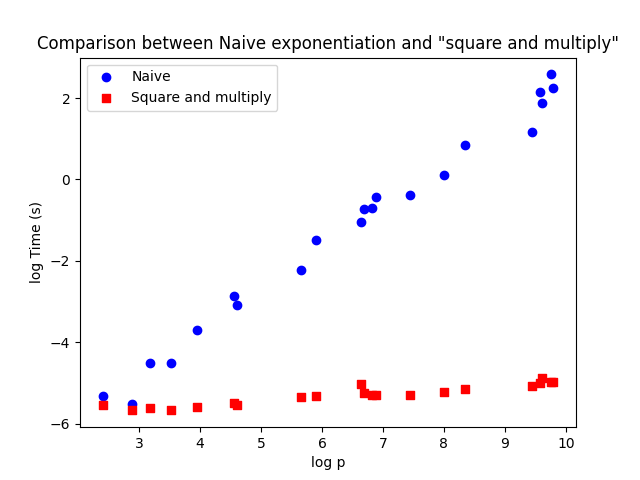
\includegraphics[width=0.5\linewidth]{plot_2025-01-24 14-39-00_0.png}
    \caption{Measurements}
    \label{figure1}
\end{figure}


\section*{References}
If applicable, include references to books, articles, or websites used in your research. For example:
\begin{enumerate}
    \item Author, Title, Year.
    \item Website Name, \texttt{www.example.com}.
\end{enumerate}

\end{document}
